\documentclass[11pt,letterpaper]{report}
\newcommand{\Empresa}{Synaptix}
\newcommand{\EmpresaArchivo}{SYNAPTIX}
\newcommand{\NombreOferta}{Puerto Deportivo Bahía Panitao}
\newcommand{\VersionDocumento}{0.1}
\newcommand{\FechaDocumento}{[PENDIENTE]}
\newcommand{\ClasificacionDocumento}{Confidencial}

\usepackage{estilo/propuesta-tecnica}
% Portada vectorial reutilizable. No requiere una imagen de fondo.
\NewDocumentCommand{\PortadaPropuesta}{m m}{%
  \begin{titlepage}
    \thispagestyle{empty}
    \begin{tikzpicture}[remember picture,overlay]
      \fill[SynNavy] (current page.south west) rectangle (current page.north east);
      \fill[SynNavyLight,opacity=.52]
        ($(current page.north east)+(-4.2cm,0)$) rectangle (current page.south east);

      % Red de conexiones inspirada en la identidad digital de Synaptix.
      \draw[SynCyan,line width=2.2pt,opacity=.92]
        ($(current page.south west)+(8.2cm,2.2cm)$)
        .. controls +(3.4cm,4.0cm) and +(-4.4cm,-3.0cm) ..
        ($(current page.north east)+(-1.0cm,-4.2cm)$);
      \draw[SynBlue,line width=1.2pt,opacity=.78]
        ($(current page.south west)+(10.0cm,0.4cm)$)
        .. controls +(1.0cm,5.7cm) and +(-3.3cm,-1.0cm) ..
        ($(current page.east)+(0cm,3.0cm)$);
      \draw[SynTeal,line width=1.25pt,opacity=.70]
        ($(current page.south west)+(6.4cm,5.0cm)$)
        .. controls +(4.2cm,2.4cm) and +(-2.2cm,-4.0cm) ..
        ($(current page.north east)+(-2.0cm,-1.0cm)$);
      \draw[SynCyan!65,line width=.8pt,opacity=.62]
        ($(current page.south west)+(11.4cm,3.0cm)$)
        .. controls +(2.6cm,2.8cm) and +(-1.5cm,-3.2cm) ..
        ($(current page.north east)+(-.4cm,-7.8cm)$);

      \foreach \p/\s in {
        {($(current page.south west)+(8.2cm,2.2cm)$)}/3.2pt,
        {($(current page.south west)+(11.0cm,6.2cm)$)}/4.2pt,
        {($(current page.east)+(-1.3cm,3.0cm)$)}/3.2pt,
        {($(current page.north east)+(-2.0cm,-1.0cm)$)}/4.4pt,
        {($(current page.north east)+(-1.0cm,-4.2cm)$)}/5.0pt,
        {($(current page.north east)+(-.4cm,-7.8cm)$)}/3.1pt
      }{
        \fill[SynCyan] \p circle (\s);
        \draw[SynCyan!45,line width=.7pt] \p circle ({\s+3.2pt});
      }

      \node[anchor=north west] at ($(current page.north west)+(1.55cm,-1.35cm)$)
        {\fontsize{18}{20}\selectfont\textbf{\textcolor{SynWhite}{SYNAP}\textcolor{SynCyan}{TIX}}};
      \node[anchor=north east,text=SynCyan] at ($(current page.north east)+(-1.45cm,-1.46cm)$)
        {\fontsize{9}{11}\selectfont\bfseries INTEGRACIÓN · DATOS · DECISIONES};

      \node[anchor=west,align=left,text width=.66\paperwidth]
        at ($(current page.west)+(1.55cm,2.7cm)$) {%
          {\fontsize{13}{16}\selectfont\bfseries\textcolor{SynCyan}{PROPUESTA}}\\[2mm]
          {\fontsize{34}{38}\selectfont\bfseries\textcolor{SynWhite}{TÉCNICA}}\\[7mm]
          {\fontsize{12}{15}\selectfont\textcolor{SynWhite!82}{\NombreOferta}}
        };

      \node[anchor=west,align=left,text width=.68\paperwidth]
        at ($(current page.west)+(1.55cm,-1.0cm)$) {%
          {\fontsize{10}{12}\selectfont\bfseries\textcolor{SynCyan}{SUBDOCUMENTO #1}}\\[2mm]
          {\fontsize{19}{23}\selectfont\bfseries\textcolor{SynWhite}{#2}}
        };

      \draw[SynCyan,line width=1.5pt]
        ($(current page.south west)+(1.55cm,3.25cm)$) -- ++(3.2cm,0);
      \node[anchor=south west,align=left,text=SynWhite!74]
        at ($(current page.south west)+(1.55cm,1.35cm)$) {%
          \fontsize{9}{12}\selectfont
          \textbf{Versión} \VersionDocumento\quad
          \textbf{Fecha} \FechaDocumento\quad
          \textbf{Clasificación} \ClasificacionDocumento\\[2mm]
          \textbf{Firmante autorizado:} \FirmanteDocumento
        };
    \end{tikzpicture}
    \null
  \end{titlepage}
  \clearpage
}

\NewDocumentCommand{\FilaDeclaracionIA}{m m m m m m}{%
  #1 & #2 & #3 & #4 & #5 & #6 \\
  \hline
}

\providecommand{\DeclaracionesIA}{}

\newenvironment{declaracionia}{%
  \begingroup
  \setlength{\tabcolsep}{3pt}
  \begin{longtable}{L{\dimexpr.105\textwidth-2\tabcolsep\relax}L{\dimexpr.14\textwidth-2\tabcolsep\relax}L{\dimexpr.21\textwidth-2\tabcolsep\relax}L{\dimexpr.115\textwidth-2\tabcolsep\relax}L{\dimexpr.14\textwidth-2\tabcolsep\relax}L{\dimexpr.29\textwidth-2\tabcolsep\relax}}
    \caption{Declaración de uso de IA por sección y archivo asociado}
    \label{tab:declaracion-ia} \\
    \hline
    \EncabezadoTabla{Sección} &
    \EncabezadoTabla{Herramienta} &
    \EncabezadoTabla{Finalidad del uso} &
    \EncabezadoTabla{Nivel en texto} &
    \EncabezadoTabla{Nivel en diagramas} &
    \EncabezadoTabla{Revisión humana: responsable y verificación} \\
    \hline
    \endfirsthead
    \hline
    \EncabezadoTabla{Sección} &
    \EncabezadoTabla{Herramienta} &
    \EncabezadoTabla{Finalidad del uso} &
    \EncabezadoTabla{Nivel en texto} &
    \EncabezadoTabla{Nivel en diagramas} &
    \EncabezadoTabla{Revisión humana: responsable y verificación} \\
    \hline
    \endhead
}{%
  \end{longtable}
  \endgroup
}

\newcommand{\CierreSubdocumento}{%
  \clearpage
  \printbibliography[heading=referenciassynaptix,title={Referencias}]
  \clearpage
  \chapter*{Declaración de uso de IA}
  \addcontentsline{toc}{chapter}{Declaración de uso de IA}
  \markboth{Declaración de uso de IA}{Declaración de uso de IA}
  Synaptix registra por sección las herramientas de IA generativa utilizadas, su finalidad, el grado de intervención y la revisión humana. Ninguno indica ausencia de uso. En texto, Bajo corresponde a corrección de redacción; Medio, a borradores reescritos y verificados por el equipo; Alto, a generación sustancial. En diagramas, Bajo corresponde a sugerencias de formato; Medio, a generación asistida desde un modelo del equipo; Alto, a generación sustancial. Esta declaración deberá consolidarse en el Formulario A-6 y no reduce la responsabilidad de Synaptix por la exactitud y coherencia de la propuesta.

  Ulysses Barreto, Líder Funcional, revisó la innovación de servicio. La revisión del programa de invernada y del ingreso documental asistido se identifica en las filas correspondientes al equipo de Synaptix. José Lara, Líder de Operación / SRE, es responsable de las innovaciones de contratación y sostenibilidad. OpenAI Codex apoyó la redacción, las métricas, el diseño de incorporación, los diagramas, la concordancia del T-19, las referencias y la presentación.

  La Tabla~\ref{tab:declaracion-ia} registra el uso declarado por sección y formulario asociado.
  \begin{declaracionia}
    \DeclaracionesIA
  \end{declaracionia}
  \FuenteTabla{Registro de uso de IA de este subdocumento.}
  \par
  El control previo a la emisión comprende la identificación de los revisores, la coherencia entre el capítulo y el T-19 y la aprobación de los cambios. Las metas y las valoraciones de riesgo son propuestas; su evaluación se realizará en el piloto.
}

\graphicspath{{figuras/}}
\renewcommand{\DeclaracionesIA}{%
  \FilaDeclaracionIA{13.1}{OpenAI Codex}{Redacción y contraste con las Bases}{Alto}{Alto}{[PENDIENTE: responsable; validar problema, piloto y figura]}
  \FilaDeclaracionIA{13.2}{OpenAI Codex}{Redacción y contraste con las Bases}{Alto}{Ninguno}{[PENDIENTE: responsable; validar reglas y métricas]}
  \FilaDeclaracionIA{13.3}{OpenAI Codex}{Redacción y revisión técnica}{Alto}{Ninguno}{[PENDIENTE: responsable; validar arquitectura y piloto]}
  \FilaDeclaracionIA{13.4}{OpenAI Codex}{Redacción y revisión contractual}{Alto}{Ninguno}{[PENDIENTE: responsable; validar compatibilidad contractual]}
  \FilaDeclaracionIA{13.5}{OpenAI Codex}{Redacción y contraste ambiental}{Alto}{Ninguno}{[PENDIENTE: responsable; validar evidencia e indicadores]}
  \FilaDeclaracionIA{T-19}{OpenAI Codex}{Preparación de fichas independientes}{Alto}{Ninguno}{[PENDIENTE: responsable; verificar cinco fichas]}
}

\begin{document}
\PortadaPropuesta{13}{Cartera de innovaciones}
\pagenumbering{arabic}
\setcounter{page}{1}
\tableofcontents
\clearpage
\setcounter{chapter}{12}
\chapter{Introducción a las Innovaciones}

Synaptix propone cinco innovaciones para Bahía Panitao, una por cada tipo exigido en las Bases Administrativas \parencite[arts.~28--30, pp.~19--20]{bases-admin}. Cada una parte de un problema del puerto, identifica el aporte que excede las funciones obligatorias y define cómo se medirá el beneficio. Este capítulo busca explicar las 5 innovaciones junto a su descripción, problema que resuelven, tecnología, incorporación, impacto económico y el indicador de verificación del beneficio. Las fichas de cada innovación con todos los detalles solicitados se presentan en el Formulario T-19.

La madurez de las cuatro integraciones tecnológicas se expresa mediante la escala de nueve niveles de madurez tecnológica (\textit{Technology Readiness Levels}, TRL) de la NASA. La escala describe el avance desde la observación de principios científicos hasta la demostración de una tecnología en operación: TRL 1 corresponde a principios básicos observados; TRL 2, a un concepto o aplicación tecnológica formulados; TRL 3, a una prueba de concepto analítica o experimental; TRL 4, a la validación de componentes en laboratorio; TRL 5, a la validación de componentes en un entorno pertinente; TRL 6, a la demostración de un modelo o prototipo en dicho entorno; TRL 7, a la demostración de un prototipo en un entorno operacional; TRL 8, a un sistema completo y calificado mediante pruebas; y TRL 9, a un sistema probado satisfactoriamente en operación \parencite{nasa-trl}.

\newpage

\section{Innovación 1}




La innovación propuesta corresponde a un producto o servicio de base tecnológica denominado \textit{Servicio de Solicitud y Seguimiento de Mantenimiento de Embarcaciones}. Su objetivo es facilitar que el armador solicite trabajos de mantenimiento, que el contratista registre su respuesta y avance, y que la marina y el armador pueda consultar el estado de cada solicitud. 

\subsection{ Problema u oportunidad concreta}

Las Bases Técnicas describen un modelo en que los trabajos de mantenimiento de las embarcaciones son realizados por contratistas independientes. Además, identifican un ecosistema de 62 contratistas y aproximadamente 140 personas vinculadas a su operación \parencite{caso07}. Estas cifras dimensionan la cantidad de actores externos que pueden intervenir en la prestación de servicios, aunque no permiten afirmar que todos ellos realicen trabajos de mantenimiento. La solución base de esta propuesta toma en consideración el requisito RF-CTR-04 (Véase formulario T-12) y asignar un acceso a una orden de trabajo en la marina a un contratista específico, pero no existe trazabilidad de la marina ni del armador del estado de la orden de trabajo del contratista para ver el progreso.

La oportunidad consiste en dar trazabilidad al ciclo de una solicitud de mantenimiento entre el armador, la marina y el contratista: desde su envío y aceptación o rechazo hasta la actualización de su avance y cierre. Las bases no entregan una línea base cuantitativa sobre solicitudes sin respuesta, tiempos de coordinación o atrasos atribuibles a falta de seguimiento; estos datos deberán levantarse para estimar el problema actual y comprobar el beneficio.

\subsection{Tecnología, práctica o modelo que la sustenta}

El servicio utilizará un flujo digital de solicitudes y órdenes de trabajo. El armador seleccionará su embarcación y registrará los trabajos requeridos, su descripción, disponibilidad y antecedentes de apoyo. La marina revisará la solicitud y la derivará al contratista pertinente. Este podrá aceptarla o rechazarla y, si la acepta, proponer una fecha.

La figura 13.1  representa el flujo de estados de la innovación: \textit{Enviada}, \textit{En revisión}, \textit{Pendiente de respuesta}, \textit{Aceptada}, \textit{Rechazada}, \textit{Programada}, \textit{En ejecución}, \textit{En espera}, \textit{Finalizada}, \textit{Cerrada} y \textit{Cancelada}. Cada cambio conservará el estado anterior y nuevo, la fecha y hora, el usuario responsable y, cuando corresponda, el motivo. Se emitirán notificaciones al armador cuando cambie el estado de su solicitud.



% En el documento
\begin{figure}[H]
  \centering
  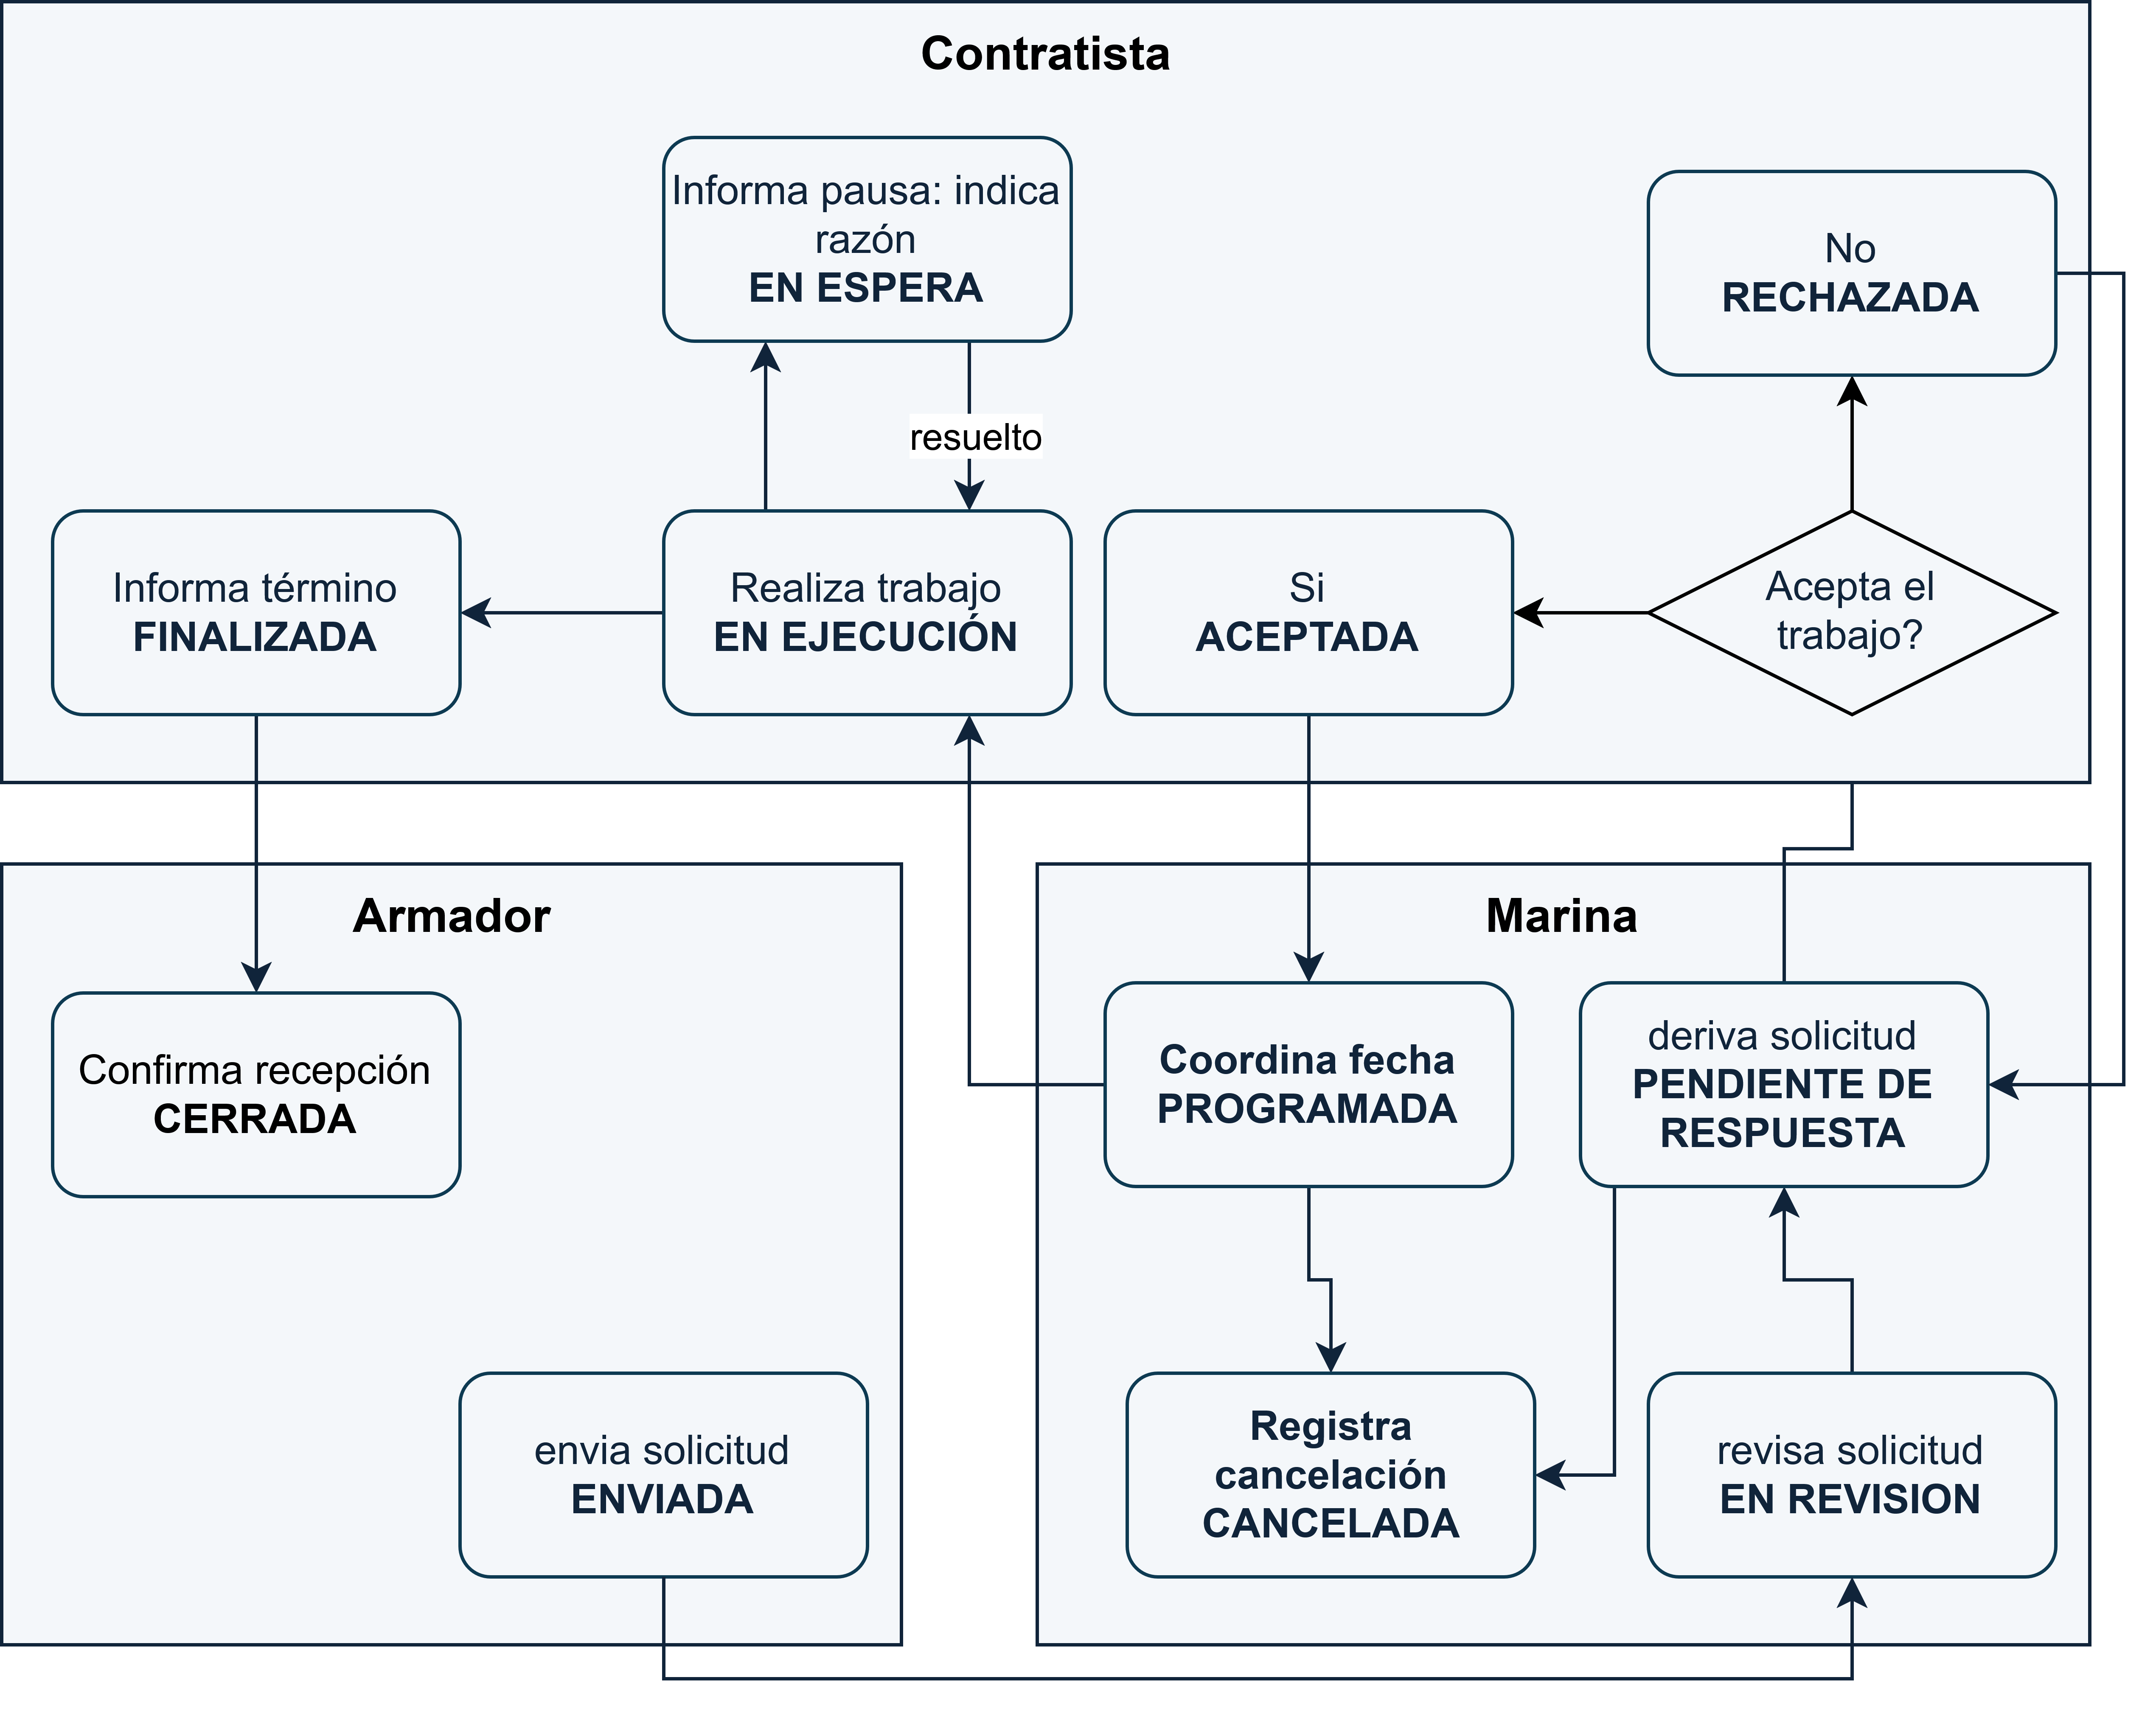
\includegraphics[width=\textwidth]{figuras/fig innov1 .png}
  \caption{Flujo de estados de la solicitud de mantenimiento}
  \label{fig:mi-imagen}
\end{figure}

el diagrama presenta el flujo de una solicitud de mantenimiento y las responsabilidades del armador, la marina y el contratista. El proceso comienza cuando el armador envía una solicitud, que pasa al estado \textit{Enviada}. Luego, el responsable de la marina la revisa y la deriva a un contratista, quedando \textit{Pendiente de respuesta}.

El contratista evalúa si puede realizar el trabajo. Si lo rechaza, la solicitud vuelve a la marina para que esta pueda derivarla a otro contratista. Si la acepta, queda \textit{Aceptada} y la marina coordina con el contratista una fecha de atención, registrándola como \textit{Programada}. Al comenzar los trabajos, el contratista actualiza la solicitud a \textit{En ejecución}. Si debe interrumpirlos, informa el motivo y la solicitud pasa a \textit{En espera}; una vez resuelta la causa, el trabajo retoma el estado \textit{En ejecución}.


La solución no asignará automáticamente contratistas ni certificará los trabajos ejecutados. La aceptación, programación y actualización del trabajo corresponderán a los actores responsables. Los estados son recopilados de sistemas de ordenes de trabajo para seguir actividades de mantenimiento \parencite{ibm-work-orders,ibm-work-order-statuses}.

\subsection{Nivel de madurez de la tecnología o práctica}

Para el Servicio de Solicitud y Seguimiento de Mantenimiento, se cataloga como TRL 2 de forma preliminar: el flujo y su aplicación a la marina están definidos conceptualmente, pero aún no se han implementado ni probado con armadores, personal de la marina y contratistas. La escala se aplica al servicio integrado para este caso, no a sus componentes tecnológicos —formularios, roles, estados y notificaciones— que ya se usan en otros sistemas. Si se construye y prueba un prototipo, podría evaluarse si corresponde avanzar a TRL 3 o 4; no se asigna ese nivel por anticipado.

\subsection{Diseño de la incorporación}

\textbf{Arquitectura.} Se propone incorporar el flujo como una extensión asociada a los módulos VAR (Varadero, Travelift e Invernada), CTR (Contratistas y Control de Acceso), AUT (Portales de Autoatención), ALE (Alertas y Marejadas) y ADM (Administración Funcional e Identidad). La vinculación específica y los contratos de interfaz deberán confirmarse con la arquitectura del proyecto. La innovación se limitará a la solicitud de mantenimiento del armador y su seguimiento; no duplicará la gestión de estadías del varadero ni el registro general de contratistas.

\textbf{Paquetes de la EDT.} La incorporación requiere, como mínimo, paquetes de trabajo para:
\begin{itemize}
    \item diseño del flujo, los estados y las reglas de transición;
    \item desarrollo de formularios para crear y consultar solicitudes;
    \item gestión de roles, historial y notificaciones;
    \item integración con los módulos correspondientes;
    \item pruebas funcionales y de aceptación;
    \item capacitación y ejecución del piloto.
\end{itemize}
Los códigos de estos paquetes quedan \textbf{pendientes de conciliación con la EDT aprobada}.

\textbf{Mes de materialización.} El mes de diseño, el período de desarrollo, el piloto y la aceptación quedan \textbf{pendientes de alinear con el cronograma base}. No se asigna un mes sin revisar la planificación vigente.

\subsection{Impacto económico estimado}

La inversión incremental comprenderá el diseño del flujo, desarrollo, integración, pruebas, capacitación y puesta en marcha. El costo operacional incluirá soporte, mantenimiento del servicio y envío de notificaciones. Los montos en UF quedan pendientes de estimación y deberán incorporarse al flujo de caja en los períodos correspondientes.

El beneficio esperado es reducir el tiempo que la marina dedica a coordinar y responder consultas sobre solicitudes, además de facilitar la detección de trabajos pendientes o detenidos. Para estimarlo, se propone medir el volumen de solicitudes y las horas de coordinación antes y después del piloto. El beneficio económico podrá calcularse como:

\[
B_t =
\left(H_{\mathrm{base},t} - H_{\mathrm{posterior},t}\right)
\times C_{\mathrm{hora}}
-
C_{\mathrm{operación},t},
\]

donde \(H_{\mathrm{base},t}\) representa las horas de coordinación antes del servicio, \(H_{\mathrm{posterior},t}\) las horas observadas después de su puesta en marcha y \(C_{\mathrm{hora}}\) el costo horario asociado. La inversión y los costos de operación deberán registrarse como egresos incrementales en el flujo de caja. No se atribuirán ahorros o ingresos hasta contar con mediciones que los respalden.

\subsection{Indicador de verificación del beneficio}

El indicador principal será la **mediana del tiempo transcurrido entre el envío de una solicitud y la primera respuesta del contratista**, medida en horas:

\[
T_{\mathrm{respuesta}} =
\operatorname{mediana}
\left(
t_{\mathrm{primera\ respuesta}} -
t_{\mathrm{envío}}
\right).
\]

La línea base se obtendrá de una muestra de solicitudes gestionadas antes del piloto. Si no existen registros históricos comparables, se levantará una línea base prospectiva durante un período inicial acordado con la marina. Como meta preliminar del piloto, se propone reducir la mediana del tiempo de primera respuesta en un 20\,\% respecto de la línea base; esta meta deberá validarse una vez medido el valor inicial.

La medición se realizará durante el piloto y al cierre del período de evaluación. Como indicador complementario de integridad, se verificará que el 100\,\% de las solicitudes gestionadas por el nuevo flujo conserve el estado, la fecha de actualización y el responsable de cada transición.

\subsection{ Riesgo de adopción}

Existe el riesgo de que algunos contratistas no actualicen oportunamente las solicitudes o continúen coordinando exclusivamente por teléfono o mensajería. También puede haber baja adopción por parte de los armadores, lo que produciría historiales incompletos y reduciría la utilidad del seguimiento.

Para mitigar este riesgo, se validarán los estados y responsabilidades con la marina, los armadores y los contratistas participantes; se capacitará a los usuarios del piloto y se acordará quién debe actualizar cada etapa. Si un contratista no utiliza directamente el sistema, la marina podrá registrar la respuesta recibida por el canal acordado, dejando constancia de quién ingresó la información, cuándo lo hizo y cuál fue su fuente.

\section{Innovación 2}

La innovación propuesta corresponde a una innovación de proceso denominada
\textit{Programa de Mantenimiento Preventivo en Invernada}. Su objetivo es que la marina aproveche los meses en que las embarcaciones permanecen fuera del agua para planificar, junto con cada armador, los trabajos de mantenimiento
preventivo y distribuirlos a lo largo del invierno, de modo que cada embarcación llegue a su turno de botadura con esos trabajos terminados.

\subsection{Problema u oportunidad concreta}
 
Las Bases Técnicas describen una explanada de invernada con 180 puestos en seco,de los cuales 152 estuvieron ocupados en el invierno de 2026. Las embarcaciones salen del agua entre abril y mayo y vuelven a entrar entre septiembre y noviembre, el 62~\% de los 1.150 movimientos anuales del travelift se concentraen esas dos campañas de seis semanas. Mientras la embarcación está en tierra, su armador contrata por su cuenta trabajos de casco, pintura, motor, velas o electrónica, que ejecutan empresas contratistas externas en los 14 puestos de trabajo del varadero.
 
Cada armador decide qué trabajos contratar y cuándo, sin un calendario común y sin relación con el orden en que su embarcación saldrá de la explanada, que es el que determina la  secuencia de botadura, una embarcación ubicada al fondo no puede botarse antes que las que tiene delante. A esto se suma que la operadora de charter, con 14 embarcaciones basadas en la marina, necesita que cada una esté lista, con el chequeo hecho, cuando llegan sus tripulaciones.
 
La oportunidad consiste en convertir un período en que la embarcación ya está en seco (cuando revisar el casco, cambiar ánodos o renovar la pintura
antiincrustante no exige una varada adicional), en un ciclo de mantenimiento
planificado. Las Bases no entregan una línea base sobre cuántos trabajos se
contratan durante la invernada, en qué semanas se concentran ni cuántas
embarcaciones llegan a su botadura con trabajos pendientes, estos datos deberán
levantarse para estimar el problema actual y comprobar el beneficio.

\subsection{Tecnología, práctica o modelo que la sustenta}
 
La innovación se basa en una forma de trabajo que se llama \emph{mantenimiento preventivo}. Cuando el mantenimiento preventivo se realiza en fechas fijadas de antemano, en lugar de esperar a que alguien se acuerde de hacerlo, se habla de \emph{mantenimiento programado}. Esta es la terminología que utiliza la norma europea de mantenimiento UNE-EN 13306:2018 . 
 
En una embarcación, varias de estas tareas solo pueden hacerse con el casco
fuera del agua. Por ejemplo: antes de volver a poner una embarcación en el agua
se recomienda revisar la pintura antiincrustante, que evita que algas y otros
organismos marinos se adhieran al casco, cambiar los ánodos, piezas de metal
que se desgastan a propósito para proteger de la corrosión a la hélice y a
otras partes metálicas, cuando ya están gastados en más de la mitad, y revisar
mangueras, válvulas del casco y hélices. Durante la
invernada, la embarcación ya permanece varios meses en tierra, por lo que es el
momento natural para hacer estos trabajos sin tener que sacarla del agua una
vez más.
 
El proceso se organiza en cuatro etapas que siguen el calendario de la
invernada:
 
\begin{enumerate}
  \item \textbf{Ficha de ingreso} (abril-mayo): Una vez que la embarcación
        queda apoyada en sus calzos (nunca durante la maniobra de izaje), el
        armador completa o confirma una ficha breve: tipo de embarcación y de
        propulsión, fecha de la última renovación de pintura antiincrustante y
        de ánodos, horas de motor declaradas y trabajos que ya tenga previstos.
  \item \textbf{Propuesta y aceptación} (mayo-junio): Con esa ficha y un
        catálogo de tareas preventivas por tipo de embarcación (definido con el
        encargado de varadero y las empresas contratistas), el sistema propone
        un paquete de trabajos. El armador elige qué tareas contratar y con qué
        empresa acreditada, o rechaza la propuesta completa.
  \item \textbf{Calendario de invernada} (junio-agosto): La marina distribuye
        los trabajos aceptados por semana, da prioridad a las embarcaciones que
        saldrán primero de la explanada y considera la disponibilidad de
        puestos de trabajo y de empresas con acreditación vigente. Cada trabajo
        aceptado genera una solicitud en el flujo de la Innovación~1, que
        registra su avance hasta el cierre.
  \item \textbf{Revisión de cierre} (agosto-septiembre): Tres semanas antes
        del inicio de la campaña de botadura (plazo configurable), el
        sistema identifica las embarcaciones con trabajos pendientes y notifica
        al armador y al contratista. Con esa información, la marina acuerda con
        el armador una nueva fecha para el trabajo o un ajuste de su turno de
        botadura antes de fijar la secuencia definitiva.
\end{enumerate}
 
La figura~\ref{fig:inn2-ciclo} representa el ciclo completo y distingue las
funciones que ya forman parte de la solución base de las que agrega esta
innovación.
 
\begin{figure}[H]
  \centering
  \definecolor{innNavy}{HTML}{0B2A4A}
  \definecolor{innHead}{HTML}{E3F1F9}
  \definecolor{innLaneA}{HTML}{F4F7FA}
  \definecolor{innLaneB}{HTML}{FFFFFF}
  \definecolor{innLine}{HTML}{9AAFC3}
  \definecolor{innOld}{HTML}{F1F1F1}
  \resizebox{0.99\linewidth}{!}{%
  \begin{tikzpicture}[
      font=\sffamily,
      paso/.style={draw=innNavy, line width=0.6pt, fill=white, rounded corners=2pt,
                   align=center, text width=2.4cm, minimum height=1.15cm,
                   inner sep=3pt, font=\sffamily\scriptsize, text=innNavy,
                   execute at begin node={\hyphenpenalty=10000\exhyphenpenalty=10000}},
      base/.style={paso, draw=gray!70, dashed, fill=innOld, text=black!70},
      flecha/.style={-{Stealth[length=2.2mm]}, line width=0.6pt, draw=innNavy},
      nota/.style={font=\sffamily\tiny, text=innNavy, inner sep=1pt}
    ]

    \fill[innLaneA] (0,0)     rectangle (16.4,-2.2);
    \fill[innLaneB] (0,-2.2)  rectangle (16.4,-4.4);
    \fill[innLaneA] (0,-4.4)  rectangle (16.4,-6.3);
    \foreach \y in {-2.2,-4.4} \draw[innLine, line width=0.4pt] (0,\y) -- (16.4,\y);
    \draw[innLine, line width=0.4pt] (0,0.9) rectangle (16.4,-6.3);
    \draw[innLine, line width=0.4pt] (0.9,0.9) -- (0.9,-6.3);
    \node[rotate=90, font=\sffamily\bfseries\small, text=innNavy] at (0.45,-1.1)  {Armador};
    \node[rotate=90, font=\sffamily\bfseries\small, text=innNavy] at (0.45,-3.3)  {Marina};
    \node[rotate=90, font=\sffamily\bfseries\small, text=innNavy] at (0.45,-5.35) {Contratista};
 
    \fill[innHead] (0.9,0) rectangle (16.4,0.9);
    \draw[innLine, line width=0.4pt] (0.9,0) -- (16.4,0);
    \foreach \x in {4.0,7.1,10.2,13.3} \draw[innLine, line width=0.4pt] (\x,0.9) -- (\x,0);
    \foreach \x/\etapa/\mes in {2.45/Ingreso a invernada/abr--may,
                                5.55/Propuesta/may--jun,
                                8.65/Calendario y ejecución/jun--ago,
                                11.75/Revisión de cierre/ago--sep,
                                14.85/Botadura/sep--nov}
      \node[align=center, font=\sffamily\scriptsize, text=innNavy] at (\x,0.45)
        {\textbf{\etapa}\\ \mes};
    \node[base] (M1) at (2.45,-3.3)  {Varada y registro de la posición en la explanada};
    \node[paso] (A1) at (2.45,-1.1)  {Completa la ficha de ingreso con la embarcación en calzos\\ \textbf{FICHA}};
    \node[paso] (M2) at (5.55,-3.3)  {Propone un paquete preventivo según ficha y catálogo\\ \textbf{PROPUESTA}};
    \node[paso] (A2) at (5.55,-1.1)  {Elige tareas y empresa acreditada, o rechaza\\ \textbf{ACEPTADA}};
    \node[paso] (M3) at (8.65,-3.3)  {Asigna semana y cupo según orden de botadura\\ \textbf{CALENDARIZADA}};
    \node[paso] (C3) at (8.65,-5.35) {Ejecuta y cierra cada trabajo (flujo de la Innovación~1)};
    \node[paso] (M4) at (11.75,-3.3) {Detecta trabajos pendientes antes de la campaña\\ \textbf{EN REVISIÓN}};
    \node[paso] (A4) at (11.75,-1.1) {Confirma recepción o acuerda nueva fecha};
    \node[base] (M5) at (14.85,-3.3) {Botadura según la secuencia de la explanada};
 

    \draw[flecha] (M1) -- (A1);
    \draw[flecha] (A1.east) -- (4.0,-1.1)  |- (M2.west);
    \draw[flecha] (M2) -- (A2);
    \draw[flecha] (A2.east) -- (7.1,-1.1)  |- (M3.west);
    \draw[flecha] (M3) -- (C3);
    \draw[flecha] (C3.east) -- (10.2,-5.35) |- (M4.west);
    \draw[flecha] (M4) -- node[nota, right=2pt, pos=0.3, align=left] {con\\ pendientes} (A4);
    \draw[flecha] (A4.east) -| (M5.north);
    \draw[flecha] (M4.east) -- node[nota, above=1pt, align=center] {sin\\ pendientes} (M5.west);
 
   
    \node[paso, text width=0.5cm, minimum height=0.35cm, inner sep=1pt] (L1) at (1.4,-6.85) {};
    \node[anchor=west, font=\sffamily\scriptsize, text=innNavy] at (L1.east) {Aporte de la innovación};
    \node[base, text width=0.5cm, minimum height=0.35cm, inner sep=1pt] (L2) at (6.4,-6.85) {};
    \node[anchor=west, font=\sffamily\scriptsize, text=black!70] at (L2.east) {Función de la solución base (módulo VAR)};
  \end{tikzpicture}%
  }%
  \caption{Ciclo del Programa de Mantenimiento Preventivo en Invernada}
  \label{fig:inn2-ciclo}
\end{figure}
 
El diagrama presenta el ciclo de la invernada y las responsabilidades del
armador, la marina y el contratista.
 
El proceso no obliga al armador a contratar trabajos, no elige al contratista por él, no certifica la calidad de los trabajos ejecutados y no administra la gestión interna de las empresas contratistas, exclusión ya declarada en la propuesta (RST-ALC-06). La marina coordina fechas y cupos; la contratación sigue siendo un acuerdo entre el armador y la empresa.
 







\subsection{Nivel de madurez de la tecnología o práctica}
 
El Programa de Mantenimiento Preventivo en Invernada, como proceso coordinado por la marina entre armadores y contratistas, se cataloga como TRL~2 de forma preliminar: su secuencia y sus reglas están formuladas conceptualmente, pero aún no se han implementado ni probado en Bahía Panitao. La escala se aplica al proceso integrado para este caso y no a sus componentes. Si el proceso se prueba durante una temporada de invernada completa, podría evaluarse si corresponde avanzar a TRL~3 o~4, no se asigna ese nivel por anticipado.
 

\subsection{Diseño de la incorporación}
 
\textbf{Arquitectura:} Se propone incorporar el proceso como una extensión
asociada a los módulos VAR (Varadero, Travelift e Invernada), del que toma la
posición y la secuencia de cada embarcación en la explanada; CTR (Contratistas y
Control de Acceso), del que toma la vigencia de la acreditación de cada empresa;
AUT (Portales de Autoatención), donde el armador completa la ficha y acepta el
paquete; ALE (Alertas y Marejadas), que emite las notificaciones de la revisión
de cierre; ADM (Administración Funcional e Identidad), donde se mantiene el
catálogo de tareas. Como la marina no cuenta con personal de tecnologías de
información, el catálogo y sus parámetros (tareas por tipo de embarcación,
intervalos sugeridos y plazo de la revisión de cierre) deberán poder
modificarse desde la administración funcional, sin intervención de un
especialista. La innovación no duplicará la agenda del travelift ni el registro
de contratistas. La vinculación específica y los contratos de interfaz deberán
confirmarse con la arquitectura del proyecto.
 
\textbf{Paquetes de la EDT:} La incorporación requiere, como mínimo, paquetes
de trabajo para:
 
\begin{itemize}
  \item Levantamiento del catálogo de tareas preventivas con el encargado de
        varadero y las empresas contratistas.
  \item Diseño de la ficha de ingreso y de las reglas de propuesta.
  \item Desarrollo del calendario de invernada y de su vínculo con la
        secuencia de la explanada.
  \item Integración con el flujo de solicitudes de la Innovación~1 y con los
        módulos correspondientes.
  \item Pruebas funcionales y de aceptación.
  \item Capacitación y ejecución del piloto durante una temporada de invernada.
\end{itemize}
 
 
\textbf{Mes de materialización:} Esta innovación depende del calendario de la
marina. Las Bases prohíben intervenir los sistemas que afectan al varadero
durante las campañas de abril-mayo y septiembre-noviembre, además del
congelamiento total entre el 15 de diciembre y el 15 de marzo. Por ello, se propone habilitar el piloto
durante el invierno (junio-agosto), con embarcaciones que ya están en la
explanada y cuya ficha de ingreso se completaría al inicio del piloto, y medir sus resultados en la campaña de botadura siguiente. El ciclo completo, desde la ficha de ingreso en la varada, comenzaría en la campaña del año posterior.

\subsection{Impacto económico estimado}
 
La inversión contemplara el levantamiento del catálogo, el diseño
de la ficha y de las reglas, el desarrollo del calendario, la integración, las
pruebas, la capacitación y el piloto. El costo operacional incluirá la
actualización anual del catálogo, el soporte del proceso y el envío de
notificaciones. Los montos en UF quedan pendientes de estimación y deberán
incorporarse al flujo de caja en los períodos correspondientes.
 
El beneficio esperado para la marina es reducir las botaduras que deben
reprogramarse porque la embarcación mantiene trabajos pendientes. Cada
reprogramación exige volver a coordinar con el armador y el contratista, y
puede obligar a mover otras embarcaciones de la explanada para respetar la
secuencia. El beneficio económico podrá calcularse como:
\[
  B_t = \left(p_{\text{base},t} - p_{\text{posterior},t}\right)
        \times N_t \times C_{\text{reprog}} - C_{\text{operación},t},
\]
donde $p_{\text{base},t}$ es la proporción de embarcaciones que llegan a su
turno de botadura con trabajos pendientes sin el programa,
$p_{\text{posterior},t}$ la proporción observada con el programa, $N_t$ el
número de embarcaciones participantes en la temporada $t$ y
$C_{\text{reprog}}$ el costo medio de una reprogramación, que incluye las horas
de coordinación y los movimientos adicionales en la explanada. Otros beneficios
posibles, como mayores ingresos por derechos de trabajo en el varadero o
embarcaciones de charter listas a la llegada de sus tripulaciones, no se contabilizarán
mientras no pueda demostrarse que se deben al programa. No se atribuirán
ahorros o ingresos hasta contar con mediciones que los respalden.
 

\subsection{Indicador de verificación del beneficio}
 
El indicador principal será la proporción de embarcaciones que llegan a
su turno de botadura con trabajos de mantenimiento pendientes:
\[
  p_{\text{pendiente}} = \frac{N_{\text{pendientes}}}{N_{\text{con trabajos}}},
\]
donde $N_{\text{con trabajos}}$ corresponde a las embarcaciones que contrataron al menos un trabajo durante la invernada y $N_{\text{pendientes}}$ a las que, en la fecha programada de su botadura, mantienen al menos uno de esos trabajos sin cerrar.
 
Como la participación es voluntaria, la línea base se obtendrá en la misma
campaña de botadura, comparando las embarcaciones del piloto con las que no
participan y que también contrataron trabajos. Esta comparación controla el
efecto del clima y de las marejadas de esa temporada, aunque los armadores que se inscriben voluntariamente podrían ser, de por sí, más organizados, por ello, cuando existan registros de la campaña anterior, también se comparará cada embarcación del piloto con su propio historial. Como meta preliminar del piloto, se propone reducir a la mitad la proporción de embarcaciones con trabajos pendientes respecto del grupo sin programa, esta meta deberá validarse una vez medido el valor inicial.
 
La medición se realizará al cierre de la campaña de botadura siguiente al
piloto. Como indicador complementario, se medirá la proporción de trabajos del programa ejecutados entre junio y agosto, fuera de las campañas de varada y botadura. Como indicador de integridad, se verificará que el 100~\% de los trabajos aceptados quede vinculado a una solicitud con su estado de cierre y su fecha.
 

\subsection{Riesgo de adopción}
 
Existe el riesgo de que los armadores perciban la propuesta como una intromisión o como una forma de venderles servicios. En el levantamiento, un armador y accionista señaló que parte de lo que compra al pagar una amarra es que nadie lo esté mirando. También es posible que las empresas contratistas, muchas de ellas pequeñas o de un solo trabajador, no respeten las semanas asignadas, y que las marejadas, más frecuentes en invierno, cancelen jornadas de trabajo y desordenen el calendario.
 
Para mitigar estos riesgos, la participación será voluntaria y la propuesta
tendrá carácter de sugerencia, es decir, el armador decide qué contratar, con quién y cuándo, y puede retirarse en cualquier momento. El calendario reservará semanas de holgura para absorber las jornadas canceladas por marejada. Respecto de los contratistas, la semana asignada se incorporará a la orden de trabajo que la portería ya verifica antes de autorizar el ingreso, que es el punto donde la marina tiene control efectivo sobre las empresas externas. Si un contratista no usa el sistema, la marina podrá registrar el avance informado por el canal acordado, dejando constancia de su fuente. Finalmente, el piloto se ofrecerá primero a un grupo acotado de armadores voluntarios, si sus embarcaciones invernan en la marina, a la operadora de charter, que ya exige embarcaciones listas a la llegada de sus tripulaciones para ajustar el catálogo antes de extenderlo.

\newpage

\section{Innovación 3}

La innovación propuesta corresponde a la adopción de inteligencia artificial (Machine Learning) e integración documental, denominada \textbf{Lectura inteligente de documentos para el ingreso asistido de antecedentes}. El objetivo es reducir el tiempo destinado a transcribir y revisar información de los documentos que recibe la marina. El sistema extraerá campos desde archivos digitales y los presentará como una propuesta que un funcionario autorizado deberá revisar y confirmar antes de incorporarla al expediente.

\subsection{Problema u oportunidad concreta}

La solución base contempla administrar los datos maestros de armadores y embarcaciones mediante RF-ADM-01 y validar la vigencia de certificados y seguros mediante RF-NAV-11, según el Formulario T-12 del subdocumento 3. Sin embargo, estos requerimientos no especifican la extracción automática de información desde los documentos que respaldan los antecedentes. Conservar una póliza en el repositorio permite consultarla, pero obtener de ella el número, la embarcación asegurada y las fechas de vigencia sigue requiriendo un mecanismo de ingreso de datos.

La oportunidad consiste en incorporar una lectura automática que prepare esos campos para su revisión. El funcionario podrá comprobar y corregir la propuesta junto al documento original, reduciendo la transcripción y facilitando la identificación de datos faltantes o discrepantes. El aporte adicional se sitúa en la captura asistida de información documental; las validaciones de vigencia y los registros maestros seguirán siendo responsabilidad de los módulos existentes.

No se dispone de una línea base verificada sobre el volumen mensual de pólizas recibidas, su diversidad de formatos ni el tiempo necesario para ingresarlas. Estas variables se levantarán antes del piloto para dimensionar el esfuerzo actual y determinar si el beneficio esperado justifica la inversión.

\subsection{Tecnología, práctica o modelo que la sustenta}

La implementación utilizará la tecnología reconocimiento óptico de caracteres, conocido como OCR por su denominación en inglés (\textit{Optical Character Recognition}), con la extracción de campos y reglas de comprobación. El OCR reconocerá el texto de documentos escaneados o fotografías; la extracción asociará ese contenido con los campos requeridos; y las reglas identificarán datos incompletos o inconsistentes. Los resultados tendrán carácter de propuesta hasta su aprobación por el funcionario.

Se propone emplear Amazon Textract como componente de lectura y análisis documental, integrado mediante un adaptador con la plataforma. Su documentación describe la extracción de texto y formularios, las relaciones entre claves y valores, y la identificación de la página y ubicación de los elementos encontrados. Estas capacidades permiten presentar cada campo junto con el fragmento documental que lo respalda \parencite{in3-aws-analisis}.

El piloto utilizará documentos impresos en español, recibidos como PDF o imágenes legibles. La documentación de Textract admite detección de texto en español, pero restringe la funcionalidad \textit{Queries} a documentos en inglés y el reconocimiento manuscrito al inglés. Por ello, el diseño inicial utilizará OCR y extracción de formularios, complementados con reglas de identificación de campos, sin depender de \textit{Queries} para las pólizas en español. La calidad de extracción se comprobará con muestras de los formatos efectivamente utilizados por la marina \parencite{in3-aws-limites}.

El flujo se organizará en cinco pasos:

\begin{enumerate}
    \item \textbf{Recepción.} El armador o funcionario carga la póliza y selecciona la embarcación correspondiente. El sistema comprueba que el archivo tenga un formato admitido, conserva el original y registra quién lo incorporó.
    \item \textbf{Extracción.} El componente propone el número de póliza, el asegurado, la aseguradora, la identificación de la embarcación y las fechas de inicio y término de vigencia. Un campo que no pueda identificarse permanece pendiente; no se completa mediante una suposición.
    \item \textbf{Comprobación.} Las reglas detectan campos obligatorios ausentes, fechas ambiguas, vigencias incoherentes y posibles diferencias con los identificadores del expediente. Una discrepancia genera una observación para el revisor.
    \item \textbf{Revisión.} El funcionario visualiza el documento y el formulario propuesto. Al seleccionar un campo, puede consultar su fragmento de origen. Corrige los datos necesarios y confirma la asociación con la embarcación.
    \item \textbf{Incorporación.} Los valores aprobados se registran con la identificación del documento, el responsable y la fecha de aprobación. El módulo NAV aplica posteriormente las validaciones de la solución base. Una renovación conserva la relación con los antecedentes anteriores y su historial.
\end{enumerate}

Los niveles de confianza del extractor servirán para destacar campos que requieren mayor atención. No se interpretarán como garantía de exactitud y, durante el piloto, todos los documentos tendrán revisión humana. AWS recomienda considerar la sensibilidad del uso y ajustar los umbrales de confianza al contexto de la aplicación \parencite{in3-aws-practicas}.

La gestión de riesgos se sustentará en ISO/IEC 23894:2023, que proporciona orientación para integrar el tratamiento de riesgos de inteligencia artificial en las actividades de las organizaciones. Su aplicación a esta innovación comprenderá identificar errores de extracción, evaluar sus consecuencias, definir controles y revisar el desempeño del componente. La referencia al estándar no constituye una certificación ni una garantía de precisión \parencite{in3-iso23894}.

La lectura automática no acreditará la autenticidad de la póliza ni determinará por sí sola la suficiencia de su cobertura. Esas comprobaciones corresponderán a los responsables y procedimientos definidos por la marina.

\subsection{Nivel de madurez de la tecnología o práctica}

El reconocimiento de texto y la extracción de formularios cuentan con componentes comerciales disponibles, como el servicio descrito. Esta disponibilidad permite plantear una integración sobre capacidades existentes, aunque no acredita su desempeño sobre las pólizas particulares de Bahía Panitao.

Debido a lo anterior, se clasifica preliminarmente en \textbf{TRL 2}: al igual que las innovaciones anteriores su aplicación y flujo están formulados conceptualmente, pero todavía no se han implementado ni probado en la marina. La escala considera ese nivel con la formulación del concepto o aplicación tecnológica. La clasificación se refiere al componente integrado para este caso y no al servicio comercial utilizado. 

\subsection{Diseño de la incorporación}

\textbf{Arquitectura.} La innovación se incorporará mediante un componente de extracción documental conectado con los módulos AUT (Portales de Autoatención), ADM (Administración Funcional e Identidad) y NAV (Dominio Náutico y Zarpes). AUT proporcionará la carga y consulta del estado del documento; ADM gestionará permisos, campos y revisión; y NAV utilizará los antecedentes confirmados para sus validaciones. El repositorio y la auditoría existentes conservarán el original, los valores propuestos, las correcciones, la versión del procesamiento y el responsable de aprobación.

El adaptador del extractor separará la respuesta del proveedor del modelo de datos de la marina. El procesamiento se ejecutará en segundo plano, con estados visibles de pendiente, en procesamiento, pendiente de revisión, aprobado o pendiente de nueva carga. Los reintentos no deberán duplicar antecedentes ni sobrescribir registros confirmados. Si el servicio o la conexión no están disponibles, el funcionario podrá continuar con el ingreso manual previsto en la base; la extracción asistida no será una dependencia de las operaciones náuticas críticas.

Antes de habilitar el servicio se comprobarán las condiciones de tratamiento de los archivos y la compatibilidad con las restricciones de alojamiento del proyecto. Los documentos y resultados estarán sujetos a los controles de acceso, cifrado, retención y auditoría ya definidos. El alcance de esta innovación para Synaptix consta de la configuración y el mantenimiento técnico; el funcionario de la marina realizaría la revisión operacional.

\textbf{Paquetes de la EDT.} La incorporación comprenderá:
\begin{itemize}
    \item levantamiento del volumen documental, formatos y campos requeridos;
    \item preparación de muestras autorizadas y definición de reglas de comprobación;
    \item integración del extractor y desarrollo del formulario de revisión;
    \item conexión con expedientes, repositorio y auditoría;
    \item pruebas funcionales, de permisos y de continuidad ante fallos;
    \item capacitación, ejecución del piloto y evaluación del beneficio.
\end{itemize}

Los códigos de los paquetes quedan pendientes de conciliación con la EDT aprobada. El piloto se limitará a pólizas de embarcaciones; una ampliación a certificados u otros documentos requerirá comprobar su calidad de extracción y beneficio.

\textbf{Mes de materialización.} El piloto se programará una vez disponibles los expedientes, la recepción documental y las funciones de revisión requeridas, respetando las ventanas protegidas del proyecto. El mes específico queda pendiente de alineación con el cronograma base. La habilitación de la innovación no modificará los criterios de aceptación de las funciones obligatorias.

\subsection{Impacto económico estimado}

La inversión incremental comprenderá el levantamiento documental, la integración, el desarrollo de la interfaz, las pruebas y la capacitación. El costo operacional incluirá el procesamiento de documentos, el almacenamiento adicional que corresponda y el soporte de las reglas ante cambios de formato. Los montos en UF se estimarán después de medir el volumen, el número de páginas y la frecuencia de recepción; se incorporarán al flujo de caja en los períodos correspondientes.

El beneficio esperado será la reducción del tiempo de ingreso y revisión respecto del procedimiento manual dentro de la solución base. Para un período mensual $t$, se estimará como:

\[
B_t = \frac{N_t\bigl(\overline{T}_{\mathrm{base},t}
      -\overline{T}_{\mathrm{asistido},t}\bigr)}{60}
      \times C_{\mathrm{hora}}
      - C_{\mathrm{operacion},t},
\]

donde $N_t$ es el número de documentos del alcance evaluado; los tiempos promedio se expresan en minutos por documento e incluyen revisión, correcciones y tratamiento manual de los casos que no puedan extraerse; $C_{\mathrm{hora}}$ es el costo horario del personal; y $C_{\mathrm{operacion},t}$ representa el costo incremental de operación. Los promedios se utilizarán para estimar horas acumuladas, mientras que la mediana permitirá evaluar el tiempo típico de atención.

La inversión inicial se registrará separadamente como egreso. Si el ahorro corresponde a tiempo liberado de personal contratado, se presentará como capacidad operacional recuperada; solo se reconocerá un ahorro de caja cuando exista una reducción efectiva de costos. No se atribuirán a esta innovación los beneficios de digitalización ya comprometidos por la solución base.

\subsection{Indicador de verificación del beneficio}

El indicador principal será la \textbf{reducción porcentual de la mediana del tiempo total de ingreso y revisión por documento}:

\[
R_T = \frac{\mathrm{mediana}(T_{\mathrm{base}})
      -\mathrm{mediana}(T_{\mathrm{asistido}})}
      {\mathrm{mediana}(T_{\mathrm{base}})}\times 100.
\]

El tiempo se medirá desde que el funcionario comienza a ingresar o revisar el antecedente hasta que queda confirmado. Incluirá correcciones y cualquier espera que le impida continuar la tarea. La latencia completa entre carga y disponibilidad de la propuesta se registrará por separado para no ocultar demoras del procesamiento en segundo plano.

La línea base se levantará con el ingreso manual de los mismos campos requeridos en el flujo asistido. Se utilizarán muestras comparables por formato, número de páginas y legibilidad; se alternarán los métodos entre funcionarios y se evitará que una persona procese inmediatamente el mismo documento por ambos procedimientos. Los casos que requieran ingreso manual se mantendrán dentro de la evaluación del flujo asistido.

Como meta preliminar se propone reducir la mediana en un \textbf{30\,\%} respecto de la línea base, sin aumentar la tasa de errores en registros aprobados. La meta se revisará una vez medido el desempeño inicial y no representa un beneficio demostrado. El tamaño de muestra y la duración del piloto se fijarán según el volumen y la variabilidad observados.

Como indicadores complementarios se medirán la proporción de campos corregidos, el porcentaje de documentos completados manualmente, el costo por documento y los errores detectados mediante una revisión independiente de los registros aprobados. Se comprobará, además, que el 100\,\% de las aprobaciones conserve el documento de origen, la fecha y el responsable. La evaluación al cierre del piloto determinará la conveniencia de ampliar, ajustar o mantener acotada la implementación.

\subsection{Riesgo de adopción}

El riesgo de adopción se considera preliminarmente \textbf{medio}, aunque un error en la identificación de la embarcación o en la vigencia podría tener consecuencias relevantes. Fotografías deficientes, cambios de formato o confusión entre fecha de emisión y vencimiento pueden producir campos incorrectos. La mitigación consistirá en mostrar el fragmento de origen, destacar ambigüedades, contrastar identificadores y exigir confirmación antes de incorporar los antecedentes.

También existe el riesgo de que el personal acepte los datos propuestos sin revisarlos o que las correcciones consuman tanto tiempo como el ingreso manual. Se capacitará a los funcionarios sobre los límites del extractor, se revisará una muestra de registros aprobados y se analizarán los errores por campo y formato. Si un formato presenta resultados insuficientes, se mantendrá su ingreso manual mientras Synaptix ajusta y vuelve a evaluar el procesamiento.

La dependencia de un servicio externo introduce riesgos de indisponibilidad, cambios de condiciones y tratamiento de documentos fuera de las ubicaciones autorizadas. Antes de la habilitación se verificará su compatibilidad con el proyecto; el adaptador y la alternativa manual permitirán mantener el proceso si el componente no está disponible. Los permisos y la trazabilidad existentes se aplicarán también a los archivos y resultados de extracción.

Finalmente, un volumen reducido de documentos podría impedir recuperar la inversión. El piloto comenzará con un alcance acotado y la ampliación se decidirá a partir del tiempo efectivamente recuperado, la calidad de los registros y el costo incremental. Si el beneficio no se demuestra, se conservará el procedimiento manual de la solución base y se revisará la continuidad del componente adicional.
\newpage


\section{Innovación 4}

Servicio Gestionado por Resultados es una innovación de modelo de negocio o contratación. Bahía Panitao debe operar la plataforma durante 36 meses sin un área interna de informática \parencite[caps.~2 y 9]{caso07}. La operación, mesa de ayuda y niveles de servicio son obligaciones de la oferta. El aporte adicional propuesto es una fracción variable de remuneración asociada a beneficios adicionales, medidos y conciliados con el cliente. La disponibilidad contractual mantiene su régimen propio; no se redefine como innovación ni se cobra dos veces por el mismo resultado.

\paragraph{Modelo, madurez e incorporación.} Synaptix propone una tarifa base para las obligaciones del servicio y, sólo si las Bases y el contrato lo admiten, un componente variable sujeto a indicadores, reglas de atribución, topes y revisión conjunta. Las guías públicas de contratación por resultados vinculan pagos a indicadores controlables por el proveedor \parencite{uk-outcomes}. El modelo para este contrato está en diseño conceptual, sin aprobación contractual. \textbf{[PENDIENTE: cláusula habilitante, paquete EDT, mes de inicio, porcentaje y topes.]}

\paragraph{Impacto económico.} El componente variable, su límite y los costos de medición se reflejarán en el flujo de caja sin alterar garantías, multas ni tarifa base. \textbf{[PENDIENTE: inversión de medición, costo operacional, beneficio esperado y tratamiento contable.]}

\paragraph{Indicador y verificación.} El beneficio conciliado se calcula como mejora observada menos efectos externos y costo incremental, según una regla acordada para cada indicador. Se propone comenzar con correcciones manuales o tiempo de coordinación, usando los registros operacionales y un período de observación sin efecto económico. \textbf{[PENDIENTE: línea base, meta, fuente, regla de atribución y momento de medición.]}

\paragraph{Riesgo y contingencia.} Un incentivo mal diseñado podría premiar ahorro aparente a costa de seguridad o calidad. La mitigación exige condiciones de servicio mínimas, auditoría conjunta y exclusión de resultados no atribuibles. Si el mecanismo variable no es compatible con el contrato, Synaptix mantendrá la tarifa y los niveles de servicio obligatorios y usará el tablero de beneficios sólo para gestión. \textbf{[PENDIENTE: probabilidad e impacto.]}

\section{Innovación 5}

Pasaporte Ambiental Náutico es una innovación de experiencia de usuario y sostenibilidad. El caso registra tres no conformidades ambientales: residuos peligrosos sin trazabilidad completa, consumos no medidos por amarra y capacitación no acreditada para unas 140 personas contratistas \parencite[caps.~4 y 7]{caso07}. Esos tres controles son obligatorios. Synaptix añade una vista longitudinal por embarcación y faena, compara la evolución propia del consumo según días de permanencia y permite registrar acciones de reducción para usuarios autorizados. El pasaporte no emite certificaciones ambientales ni reemplaza la auditoría.

\paragraph{Tecnología, madurez e incorporación.} El historial relacionará eventos de residuos, lecturas validadas, embarcaciones, contratistas y vigencias de capacitación. Se insertará en la capa de datos y el portal autorizado, con registros de origen y permisos por actor. ISO 14031 orienta la evaluación del desempeño ambiental mediante indicadores, sin fijar por sí misma niveles de cumplimiento \parencite{iso14031}. La integración local se clasifica preliminarmente en TRL 2 \parencite{nasa-trl}. \textbf{[PENDIENTE: formato exigido por la auditoría, modelo de amenazas, paquete EDT, interfaces y mes del piloto.]}

\paragraph{Impacto económico.} La inversión comprende integración de fuentes, historial y vistas; la operación añade almacenamiento, conciliación y atención de rectificaciones. El beneficio esperado es menor esfuerzo para reunir evidencia y mejor información para reducir consumos. \textbf{[PENDIENTE: inversión, costo operacional y beneficio cuantificado.]}

\paragraph{Indicador y verificación.} El beneficio adicional se mide como embarcaciones participantes con una acción de reducción ambiental documentada a partir del pasaporte divididas por embarcaciones participantes. La integridad de residuos, consumos y acreditaciones es condición previa de calidad de datos, no el beneficio innovador. El piloto establecerá la línea base con armadores voluntarios. \textbf{[PENDIENTE: línea base, meta, tamaño de muestra y momento de medición anterior a la auditoría de 2029.]}

\paragraph{Riesgo y contingencia.} Lecturas incompletas o documentos desactualizados pueden producir un historial engañoso. Synaptix mitigará el riesgo mostrando procedencia, fecha y estado de validación de cada dato, además de conciliación manual de discrepancias. Si la vista integrada no supera el piloto, permanecerán disponibles los registros obligatorios de residuos, medición y capacitación. \textbf{[PENDIENTE: probabilidad e impacto.]}

\CierreSubdocumento
\end{document}
